\section{Обзор шардирования в СУБД Tarantool}

В этом разделе детально исследуется реализация механизма шардирования в СУБД
Tarantool. Кроме того, анализируются ключевые компоненты модуля шардирования,
понимание которых необходимо для реализации предложенного подхода к выполнению
Map запросов на репликах.

\subsection{Обзор}

В Tarantool логически связанные узлы, работающие с идентичными копиями базы
данных, объединяются в репликасеты (replicaset). В рамках каждого набора узлам
назначаются роли: мастер (master) или реплика (replica). Обработка запросов
на изменение данных (DDL, DML, DCL) осуществляется исключительно на мастере,
тогда как реплики обслуживают только запросы на чтение (DQL). Между узлами
внутри репликасета поддерживается процесс синхронизации данных посредством
репликации.

Реализация шардирования в Tarantool обеспечивается модулем \textit{vshard}
\cite{VshardGithub}, разработанным на языке Lua. Этот выбор обусловлен тем, что
Tarantool сочетает функциональность СУБД с возможностью исполнения прикладной
логики, которая реализуется на Lua.

Модуль \textit{vshard} в Tarantool обеспечивает распределение кортежей набора
данных среди нескольких шардов, представляющих собой репликасеты. Каждый шард
обрабатывает только определённое подмножество общих данных, что позволяет
масштабировать систему под повышенную нагрузку путём добавления новых шардов.

Модуль \textit{vshard} предоставляет API маршрутизатора (router) и
API хранилища (storage) для разработки приложений, поддерживающих
шардирование.

\subsection{Архитектура шардированного кластера Tarantool}

Рассмотрим распределенный кластер Tarantool, состоящий из подкластеров,
называемых шардами, каждый из которых хранит некоторую часть данных. Каждый
шард, в свою очередь, представляет собой набор реплик (replica set), состоящий
из нескольких реплик, одна из которых служит главным узлом (master node),
обрабатывающим все запросы на чтение и запись.

Весь набор данных логически разделен на заранее определенное количество
виртуальных бакетов (далее - бакеты), каждому из которых присвоен уникальный
номер в диапазоне от 1 до N, где N - общее количество бакетов. Количество
бакетов специально выбирается на несколько порядков больше потенциального
количества узлов кластера, даже с учетом будущего масштабирования кластера.
Например, при M проектируемых узлах набор данных может быть разделен на 100M
или даже 1000M бакетов. При выборе количества бакетов следует соблюдать
осторожность: если оно слишком велико, это может потребовать дополнительной
памяти для хранения информации о маршрутизации; если слишком мало, это может
уменьшить детализацию перебалансировки.

Каждый шард хранит уникальное подмножество бакетов, что означает, что бакет не
может принадлежать нескольким шардам одновременно, как показано на
рис~\ref{fig:fig03}.

\begin{figure}
  \centering
  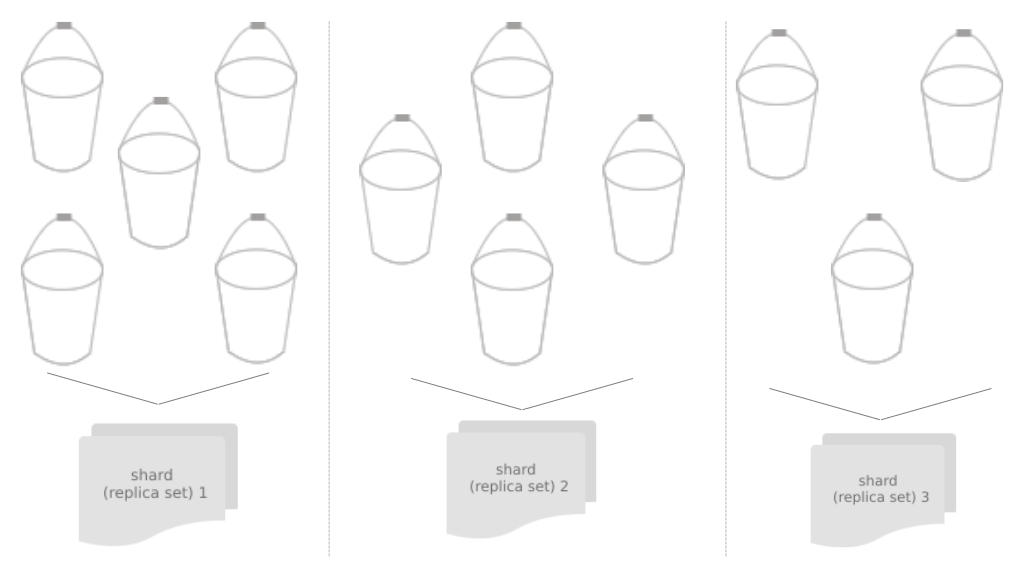
\includegraphics[scale=0.7]{inc/bucket.png}
    \caption{Виртуальные бакеты \cite{VshardDoc}}
  \label{fig:fig03}
\end{figure}

Данное соответствие шардов и бакетов хранится в таблице в одном из системных
спейсов Tarantool, причем каждый шард содержит только определенную часть этой
карты, которая покрывает те бакеты, которые были назначены данному шарду.

Помимо таблицы соответствия, идентификатор бакета также хранится в специальном
поле каждого кортежа каждой таблицы, участвующей в шардировании.

Когда шард получает любой запрос (кроме SELECT) от приложения, этот шард
проверяет идентификатор бакета, указанный в запросе, по таблице идентификаторов
бакетов, принадлежащих данному узлу. Если указанный идентификатор бакета
недействителен, запрос завершается со следующей ошибкой: "wrong bucket". В
противном случае запрос выполняется, и всем данным, созданным в процессе,
присваивается идентификатор бакета, указанный в запросе. Важно отметить, что
запрос должен изменять только те данные, которые имеют тот же идентификатор
бакета, что и сам запрос.

Хранение идентификаторов бакетов как в самих данных, так и в таблице
соответствия обеспечивает целостность данных независимо от логики приложения и
делает перебалансировку прозрачной для приложения. Хранение таблицы
соответствия в системном спейсе гарантирует согласованность шардирования в
случае отказа, поскольку все реплики в шарде разделяют общее состояние таблицы.

Шардированный кластер в Tarantool состоит из:

\begin{itemize}
    \item \textbf{Одного или нескольких наборов реплик}:
    \begin{itemize}
        \item Каждый набор реплик должен содержать как минимум два экземпляра
              хранилища (storage)
        \item Для обеспечения избыточности рекомендуется иметь 3 или более
              экземпляров хранилища в наборе реплик
    \end{itemize}

    \item \textbf{Одного или нескольких маршрутизаторов (router)}:
    \begin{itemize}
        \item Количество экземпляров маршрутизаторов не ограничено
        \item Его следует увеличивать, если существующие экземпляры
              маршрутизаторов становятся узким местом из-за нагрузки на ЦПУ или
              ввод-вывод
    \end{itemize}
    \item \textbf{Балансировщика (Rebalancer)}
\end{itemize}

Структура шардированного кластера представлена на рис~\ref{fig:fig04}

\begin{figure}
  \centering
  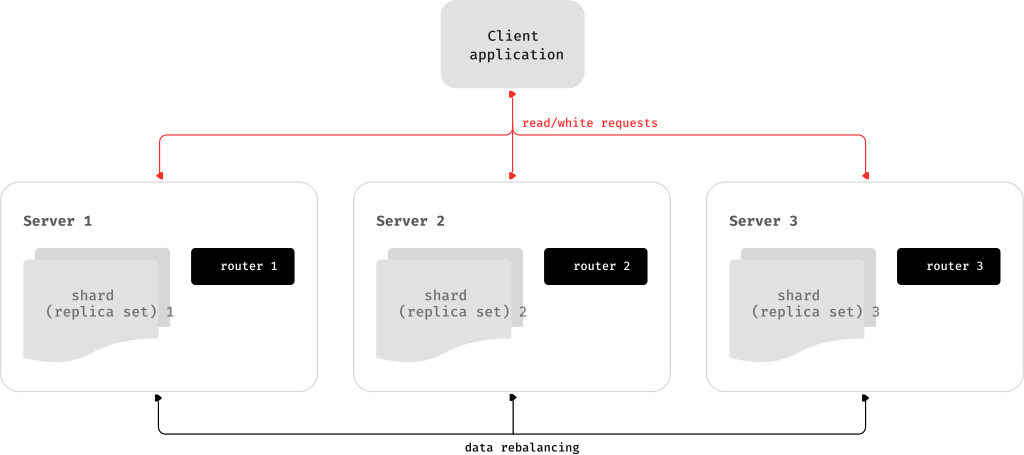
\includegraphics[scale=0.5]{inc/schema.png}
  \caption{Архитектура шардированного кластера \cite{VshardDoc}}
  \label{fig:fig04}
\end{figure}

\subsection{Маршрутизатор (router)}

Маршрутизатор (далее роутер) представляет собой автономный программный
компонент, который направляет запросы на чтение и запись от клиентского
приложения к соответствующим шардам.

Все запросы от приложения поступают в шардированный кластер через роутер.
Роутер обеспечивает прозрачность топологии шардированного кластера для
приложения, скрывая от него:

\begin{itemize}
\item количество и расположение шардов,
\item процесс перебалансировки данных,
\item факт и процесс отработки отказа при сбое реплики.
\end{itemize}

Роутер может самостоятельно вычислять идентификатор бакета при условии, что
приложение явно определяет правила вычисления идентификатора бакета на основе
данных запроса. Для этого роутер должен знать схему данных.

Роутер не имеет постоянного состояния и не хранит топологию кластера, а также
не выполняет балансировку данных. Это автономный программный компонент, который
может работать на уровне хранилища или на уровне приложения в зависимости от
особенностей приложения.

Роутер поддерживает постоянный пул соединений со всеми хранилищами, создаваемый
при запуске. Такой подход помогает избежать ошибок конфигурации. После создания
пула роутер кэширует текущее состояние спейса \texttt{\_bucket} для ускорения
маршрутизации. В случае перемещения идентификатора бакета на другое хранилище в
результате ребалансировки данных или при переходе одного из шардов на реплику,
роутер обновляет таблицу маршрутизации.

Шардирование не интегрировано в какую-либо централизованную систему хранения
конфигурации. Предполагается, что само приложение обрабатывает все
взаимодействия с такими системами и передает параметры шардирования. При этом
конфигурация может изменяться динамически - например, при добавлении или
удалении одного или нескольких шардов:

\begin{itemize}
\item Для добавления нового шарда в кластер системный администратор сначала
    изменяет конфигурацию всех роутеров, а затем конфигурацию всех хранилищ.
\item Новый шард становится доступным уровню хранилища для перебалансировки.
\item В результате перебалансировки один из виртуальных бакетов перемещается на
    новый шард.
\item При попытке доступа к виртуальному бакету роутер получает специальный код
    ошибки, указывающий новое местоположение бакета.
\end{itemize}

\subsection{Ребалансировщик}

Ребалансировщик представляет собой фоновый процесс перебалансировки, который
обеспечивает равномерное распределение бакетов между шардами. В процессе
перебалансировки происходит миграция бакетов между наборами реплик.

Балансировщик периодически "просыпается" и перераспределяет данные из наиболее
загруженных узлов в менее загруженные узлы. Перебалансировка запускается, если
дисбаланс набора реплик превышает заданный в конфигурации пороговый уровень.

Дисбаланс набора реплик рассчитывается следующим образом:
\begin{equation}
|etalon\_bucket\_number - real\_bucket\_number| / etalon\_bucket\_number * 100
\end{equation}

\subsection{Миграция бакетов}

Набор реплик, с которого выполняется миграция бакета, называется
источником (source); целевой набор реплик, на который выполняется
миграция, называется приемником (destination).

Во время миграции бакет может находиться в различных состояниях:

\begin{itemize}
\item \texttt{ACTIVE} -- бакет доступен для запросов на чтение и запись.
\item \texttt{PINNED} -- бакет заблокирован для миграции на другой набор
    реплик. В остальном заблокированные бакеты аналогичны бакетам в состоянии
        ACTIVE.
\item \texttt{SENDING} -- бакет в настоящее время копируется на набор реплик
    приемник; запросы на чтение к набору реплик источник все еще
        обрабатываются.
\item \texttt{RECEIVING} -- бакет в настоящее время заполняется; все запросы к
    нему отклоняются.
\item \texttt{SENT} -- бакет был мигрирован на набор реплик приемник. Роутер
    использует состояние SENT для вычисления нового местоположения бакета.
        Бакет в состоянии SENT автоматически переходит в состояние GARBAGE
        через 0.5 секунды.
\item \texttt{GARBAGE} -- бакет уже был мигрирован на набор реплик приемник во
    время перебалансировки; или бакет изначально находился в состоянии
        RECEIVING, но во время миграции произошла ошибка. Бакеты в состоянии
        GARBAGE удаляются сборщиком мусора.
\end{itemize}

Процесс миграции бакетов представлен на рис~\ref{fig:fig05}. Она выполняется
следующим образом:

\begin{enumerate}
\item На целевом наборе реплик (destination) создается новый бакет, которому
    присваивается состояние \texttt{RECEIVING}, начинается копирование данных,
        и бакет отклоняет все запросы.
\item Бакету в исходном наборе реплик (source) присваивается состояние
    \texttt{SENDING}, и бакет продолжает обрабатывать запросы на чтение.
\item После завершения копирования данных бакет в исходном наборе реплик
    переводится в состояние \texttt{SENT} и начинает отклонять все запросы.
\item Бакет в целевом наборе реплик переводится в состояние \texttt{ACTIVE} и
    начинает принимать все запросы.
\end{enumerate}

\begin{figure}
  \centering
  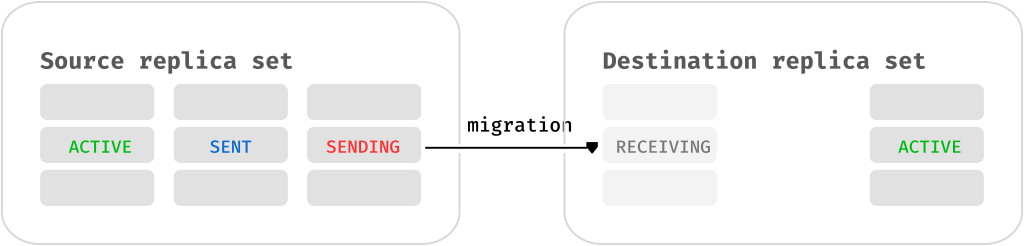
\includegraphics[scale=0.7]{inc/states.png}
  \caption{Пересылка бакета \cite{VshardDoc}}
  \label{fig:fig05}
\end{figure}

\subsection{Системный спейс \_bucket}

В системном спейсе \texttt{\_bucket} каждого набора реплик хранятся идентификаторы
бакетов, присутствующих в данном наборе реплик. Спейс содержит следующие поля:

\begin{itemize}
\item \texttt{bucket} -- идентификатор бакета
\item \texttt{status} -- состояние бакета
\item \texttt{destination} -- UUID целевого набора реплик
\end{itemize}

Пример вывода команды \texttt{\_bucket:select\{\}} представлен на рис
~\ref{fig:fig06}.

\begin{figure}
  \centering
  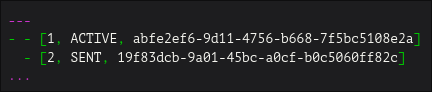
\includegraphics[scale=0.5]{inc/bucket-space.png}
  \caption{Содержание спейса \_bucket}
  \label{fig:fig06}
\end{figure}

После завершения миграции бакета в таблице заполняется поле UUID целевого
набора реплик. Пока бакет находится на исходном наборе реплик, значение UUID
целевого набора реплик равно NULL.

\subsection{Обработка запроса клиента}

Запросы к базе данных могут выполняться приложением или с использованием
хранимых процедур. В любом случае, идентификатор бакета должен быть явно указан
в запросе.

Все запросы сначала перенаправляются роутеру. Единственной операцией,
поддерживаемой роутером, является \texttt{call}. Данная операция выполняется с
помощью функции \texttt{vshard.router.call()}:

\begin{verbatim}
result = vshard.router.call(<bucket_id>, <mode>, <function_name>, \\
        {<argument_list>}, {<opts>})
\end{verbatim}

Обработка запросов выполняется следующим образом:

\begin{enumerate}
\item Роутер использует идентификатор бакета для поиска соответствующего набора
    реплик в таблице маршрутизации.
\item Если соответствие идентификатора бакета набору реплик неизвестно роутеру
    (fiber обнаружения еще не заполнил таблицу), роутер отправляет запросы ко
    всем хранилищам, чтобы определить местоположение бакета.
\item После обнаружения бакета шард проверяет:
\begin{itemize}
    \item наличие бакета в системном спейсе \texttt{\_bucket} набора реплик;
    \item находится ли бакет в состоянии \texttt{ACTIVE} или \texttt{PINNED}
        (для запросов на чтение также допустимо состояние \texttt{SENDING}).
\end{itemize}
\item Если все проверки успешны, запрос выполняется. В противном случае он
    завершается с ошибкой: "\texttt{WRONG\_BUCKET}".
\end{enumerate}
